\documentclass[../Immersed_Boundary_Method.tex]{subfiles}

\begin{document}

\section{Introduction}

\subsection{The Interpolation Function}

Given the material position $X$ we want to obtian the velocity of fluid at that point. \mn{Note that $X$ usually doesn't lies on the grid point.} This process is directly interpreted by 
\begin{equation}
    \bfu(\mathbf{X}(r, s, t), t)=\int \bfu(\mathbf{x}, t) \delta(\mathbf{x}-\mathbf{X}(r, s, t)) d \mathbf{x}
\end{equation}
\begin{wrapfigure}{l}{0.45\textwidth}
    \centering
    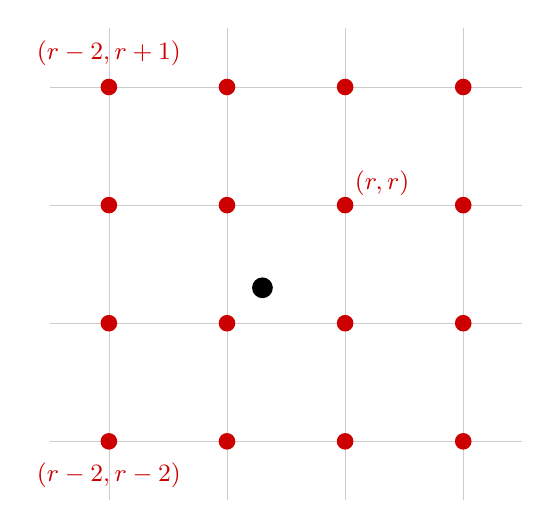
\begin{tikzpicture}[scale=1.5] % Slightly adjusted scale to fit text column better
        % 1. Draw the background grid
        \draw[step=1cm, gray!40, very thin] (-0.5,-0.5) grid (3.5,3.5);

        % 2. Draw the 4x4 grid of red points
        \foreach \x in {0,1,2,3} {
            \foreach \y in {0,1,2,3} {
                \fill[red!80!black] (\x,\y) circle (2pt);
            }
        }

        % 3. Draw the central black dot
        \fill[black] (1.3,1.3) circle (2.5pt);

        % 4. Add the labels
        % Top Left
        \node[red!80!black, above, font=\small] at (0,3.1) {$(r-2, r+1)$};
        % Inner Point
        \node[red!80!black, above right, font=\small] at (2,2) {$(r, r)$};
        % Bottom Left
        \node[red!80!black, below, font=\small] at (0,-0.1) {$(r-2, r-2)$};
    \end{tikzpicture}
\end{wrapfigure}
However in the discrete case we would need the discrete Delta Function. \par

In the figure on the left, black point is the material point and red points are the grid points. The $\delta$ function average all the velocity at the red points. \par

Something to pay attention is that in MATLAB, the convention for a matrix to represent a grid of point is to have lay points with same $x$ coordinat in the \textbf{same row} This may be different from our intuition. However, This is reasonable since we normally define the matrix for storing points to have size 
\[ N_x \times N_y\]
So it has $N_x$ rows. 


\end{document}